\chapter{Quantum Search Algorithms}

\section{Introduction}
Now we will look at another classical computing task that can be speeded up using the superposition principle. Our goal is to solve the needle in a haystack problem where we have to search for an element that satisfies a particular property that lies in a haystack of $N$ elements. Classically it seems that since this element can be any one of those $N$ elements it will take $O(N)$ steps to do this task. However the quantum algorithm, Grover's algorithm allows us to do this $O(\sqrt{N}$. Let us investigate this in detail by formulating the problem first.
\\\\
Suppose $f(x)$ is a function from $\{0, 1 \cdots, N-1\}$ to $\{0, 1\}$ Only for one value $a$, $f(a) = 1$. We seek to find this $a$. Also assume that $N = 2^n$. This way we can work with $n$ qubits (if $N$ is not of this form we can add extra elements to ensure this). Grover's algorithm involves using rotations in a 2D subspace so that this speedup ends up working.

\section{Grover's Algorithm}

Before we discuss the specifics, let us go through the main idea. Let us define two new state vectors:
$$\ket{\psi_0} = \sum_{i=0}^{N - 1} \frac{\ket{i}}{\sqrt{N}}$$ 
$$\ket{e} = \sum_{i = 0, i \neq a}^{N-1} \frac{\ket{i}}{\sqrt{N-1}}$$

Our goal is to ensure that we obtain $\ket{a}$ in the end. Notice that $$\ket{\psi_0} = \frac{\sqrt{N-1}\ket{e} + \ket{a}}{\sqrt{N}}$$ Thus $\ket{\psi_0}$ lies in the subspace spanned by $\ket{e}$ and $\ket{a}$ The coefficient of $\ket{e}$ is in general far greater than that of $\ket{a}$. Thus $\ket{\psi_0}$ will be closer to $\ket{e}$ than $\ket{a}$. Diagrammatically this can be represented as follows:
\begin{figure}[htp]
    \centering
    
\includegraphics[width=\textwidth]{twod}
\end{figure}

What we aim to do is take a vector $\ket{\psi}$ which will be initially equal to $\ket{\psi_0}$ and rotate it so that it ends up getting close to $\ket{a}$. For this what we would like to do is first reflect $\ket{\psi}$ about $\ket{e}$ and then about $\ket{\psi_0}$. Two reflections simultaneously correspond to a rotation. Reflecting about $\ket{e}$ can be done by considering an oracle that performs the operation
$$ \ket{x} \to (-1)^{f(x)}\ket{x}$$
Notice that we used a similar oracle in Deustch-Josza algoritm. Let us call this operation $O$. The way to achieve this is to take an oracle that performs the operation
$$\ket{x}\ket{y} \to \ket{x}\ket{y \oplus f(x)}$$
The construction of this oracle was described in the section on the Deustch-Josza algoritm. Let $\ket{y} = \frac{\ket{0} - \ket{1}}{\sqrt{2}}$
If $x = a$ then the oracle will perform the following operation
$$\ket{x}\ket{y} \to -\ket{x}\ket{y}$$ and for every other $x$ as $f(x) = 0$ it will preserver the state. Thus using such an oracle and simply ignoring the $\ket{y}$ qubit will allow us to get the behaviour we desire.
Now when this operation is applied on any $\ket{\psi}$ only the component along $\ket{a}$ will be flipped and the rest will remain the same. This achieves reflection about $\ket{e}$. To reflect about $\ket{\psi_0}$ we would like to use the following result that you have to prove:
\begin{exercise}
Prove that the following unitary operation $U = 2\ket{\psi}\bra{\psi} - I$ achieves reflection about the state vector $\ket{\psi}$ (Hint: take any vector in the hilbert space and write it in terms of $\ket{\psi}$ and the bases of the subspace orthogonal to  $\ket{\psi}$)
\end{exercise}

We define the Grover Operator $G$ as $$G = (2\ket{\psi_0}\bra{\psi_0} - I)O$$ This operator first reflects about $\ket{e}$ and then about $\ket{\psi_0}$
\begin{figure}[htp]
    \caption{Result after applying Grover once}
    \centering
    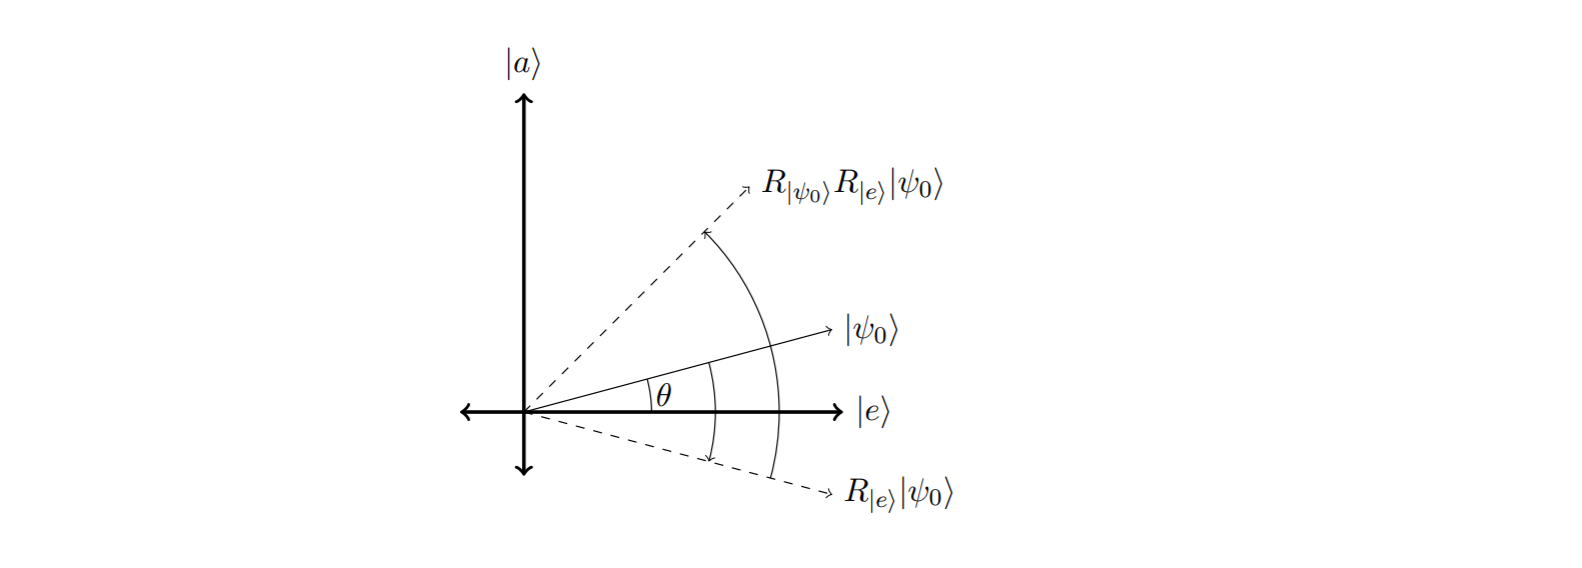
\includegraphics[width=\textwidth]{grover}
\end{figure}
Let $\psi_{0}$ make an angle $\theta$ with $\ket{e}$ in the two dimensional subspace. Then it follows that $\sin(\theta) = \frac{1}{\sqrt{N}}$. The following exercise will allow you to see how successfully applying $G$ changes our state vector which was initially $\ket{\psi_0}$

\begin{exercise}
Prove by induction that 
$$G^k \ket{\psi_0} = \cos((2k+1)\theta)\ket{e} + \sin((2k+1)\theta)\ket{a}$$
\end{exercise}

Thus applying $G$ successively on $\ket{\psi_0}$ rotates the vector by an angle $2\theta$. We can continue applying this to $\ket{\psi}$ until the angle between $\ket{\psi}$ and $\ket{a}$ will be $\leq \theta$. Then the probability of collapsing to $\ket{a}$ will be $\geq \cos(\theta) = \frac{\sqrt{N-1}}{\sqrt{N}}$. For large $N$ this will be very accurate.
How many operations of $G$ do we need though? Clearly we require $\left[ \frac{\pi}{4\theta} \right]$ applications of $G$.
Notice that $\theta \geq \sin(\theta) = \frac{1}{\sqrt{N}}$ and so 
$$\left[ \frac{\pi}{4\theta} \right] \leq \frac{\pi \sqrt{N}}{4}$$
Thus we need only $O(\sqrt{N})$ operations to achieve the task with probability $\geq \frac{\sqrt{N-1}}{\sqrt{N}}$\\\\

Thus the algorithm may be summarised as follows:\\

Algorithm: Grover's Search Algorithm\\
Input: An oracle that does the transformation $$ \ket{x} \to (-1)^{f(x)}\ket{x}$$\\
Output: The only $a$ satisfying $f(a) = 1$ with probability of success $\geq \frac{\sqrt{N-1}}{\sqrt{N}}$\\
Procedure:\\
1. Create the state $\psi_0$ by applying $H^{\otimes n}\ket{0}$\\
2. Apply the Grover operation $G = (2\ket{\psi_0}\bra{\psi_0} - I)O$ $\left[ \frac{\pi}{4\theta} \right]$ times\\
3. Measure the $n$ qubits to get $a$\\

This case of Grover's algorithm was defined when we had to search for only one element. We can modify it when multiple $x$ satisfied $f(x) = 1$ in which case we would have obtained different values of $x$ as the output (only one output per iteration of the algorithm). This modification is left as an exercise. You may want to change the two vectors that we took as the basis of the two dimension subspace over which we worked. The algorithm in this case will be $O(\sqrt{N/M})$

With this we have successfully described Grover's algorithm for searching. Although the speedup is not as significant as that in fourier transform or factoring the gains are significant. Grover's algorithm can be useful in solving $\textbf{NP Hard}$ problems by allowing us to search through the search space more quickly.

One question that may come to our minds is whether we can hope for a more significant speedup by modifying our algorithm. It has been however proven that any quantum search algorithm for the general case would still require $O(\sqrt{N})$ operations to terminate and thus Grover's algorithm is an asymptotically optimal algorithm.

